\documentclass{beamer}
%
% Choose how your presentation looks.
%
% For more themes, color themes and font themes, see:
% http://deic.uab.es/~iblanes/beamer_gallery/index_by_theme.html
%
\mode<presentation>
{
  \usetheme{Darmstadt}      % or try Darmstadt, Madrid, Warsaw, ...
  \usecolortheme{default} % or try albatross, beaver, crane, ...
  \usefonttheme{default}  % or try serif, structurebold, ...
  \setbeamertemplate{navigation symbols}{}
  \setbeamertemplate{caption}[numbered]
} 

\usepackage[english]{babel}
\usepackage[utf8x]{inputenc}

\title[Kvam Presentation 1]{Mast Cell Tumors in Guiding Eyes for the Blind Dogs}
\author{Heather McDonough, McKenzie Jones, and Stephanie Wang}
\institute{University of Richmond}
\date{\today}

\begin{document}

\begin{frame}
  \titlepage
\end{frame}

% Uncomment these lines for an automatically generated outline.
%\begin{frame}{Outline}
%  \tableofcontents
%\end{frame}

\section{Introduction}

\begin{frame}{Introduction}

%\begin{itemize}
Our lab has been working on analyzing data on mast cell cancer in Guiding Eyes for the Blind dogs using R programming. This presentation will illustrate the work we have done so far and what we hope to accomplish in the upcoming weeks. 

%\end{itemize}


\end{frame}


\subsection{Data}
\begin{frame}{Data}

We have information on over 10,000 dogs used in the Guiding Eyes for the Blind program that have been diagnosed with Mast Cell Cancer. Within this data set, we have focused on date of birth, sex, death date (if applicable), city, state, zip code, age at diagnosis, and MCT Score Value. Using this data, we have been able to create choropleth maps to illustrate where the dogs are from and ggplots to look at the correlation between date of birth and age of diagnosis in the dogs. 

\end{frame}

\subsection{Choropleth Maps}

\begin{frame}{Where The Dogs Are From}

\begin{figure}
\centering
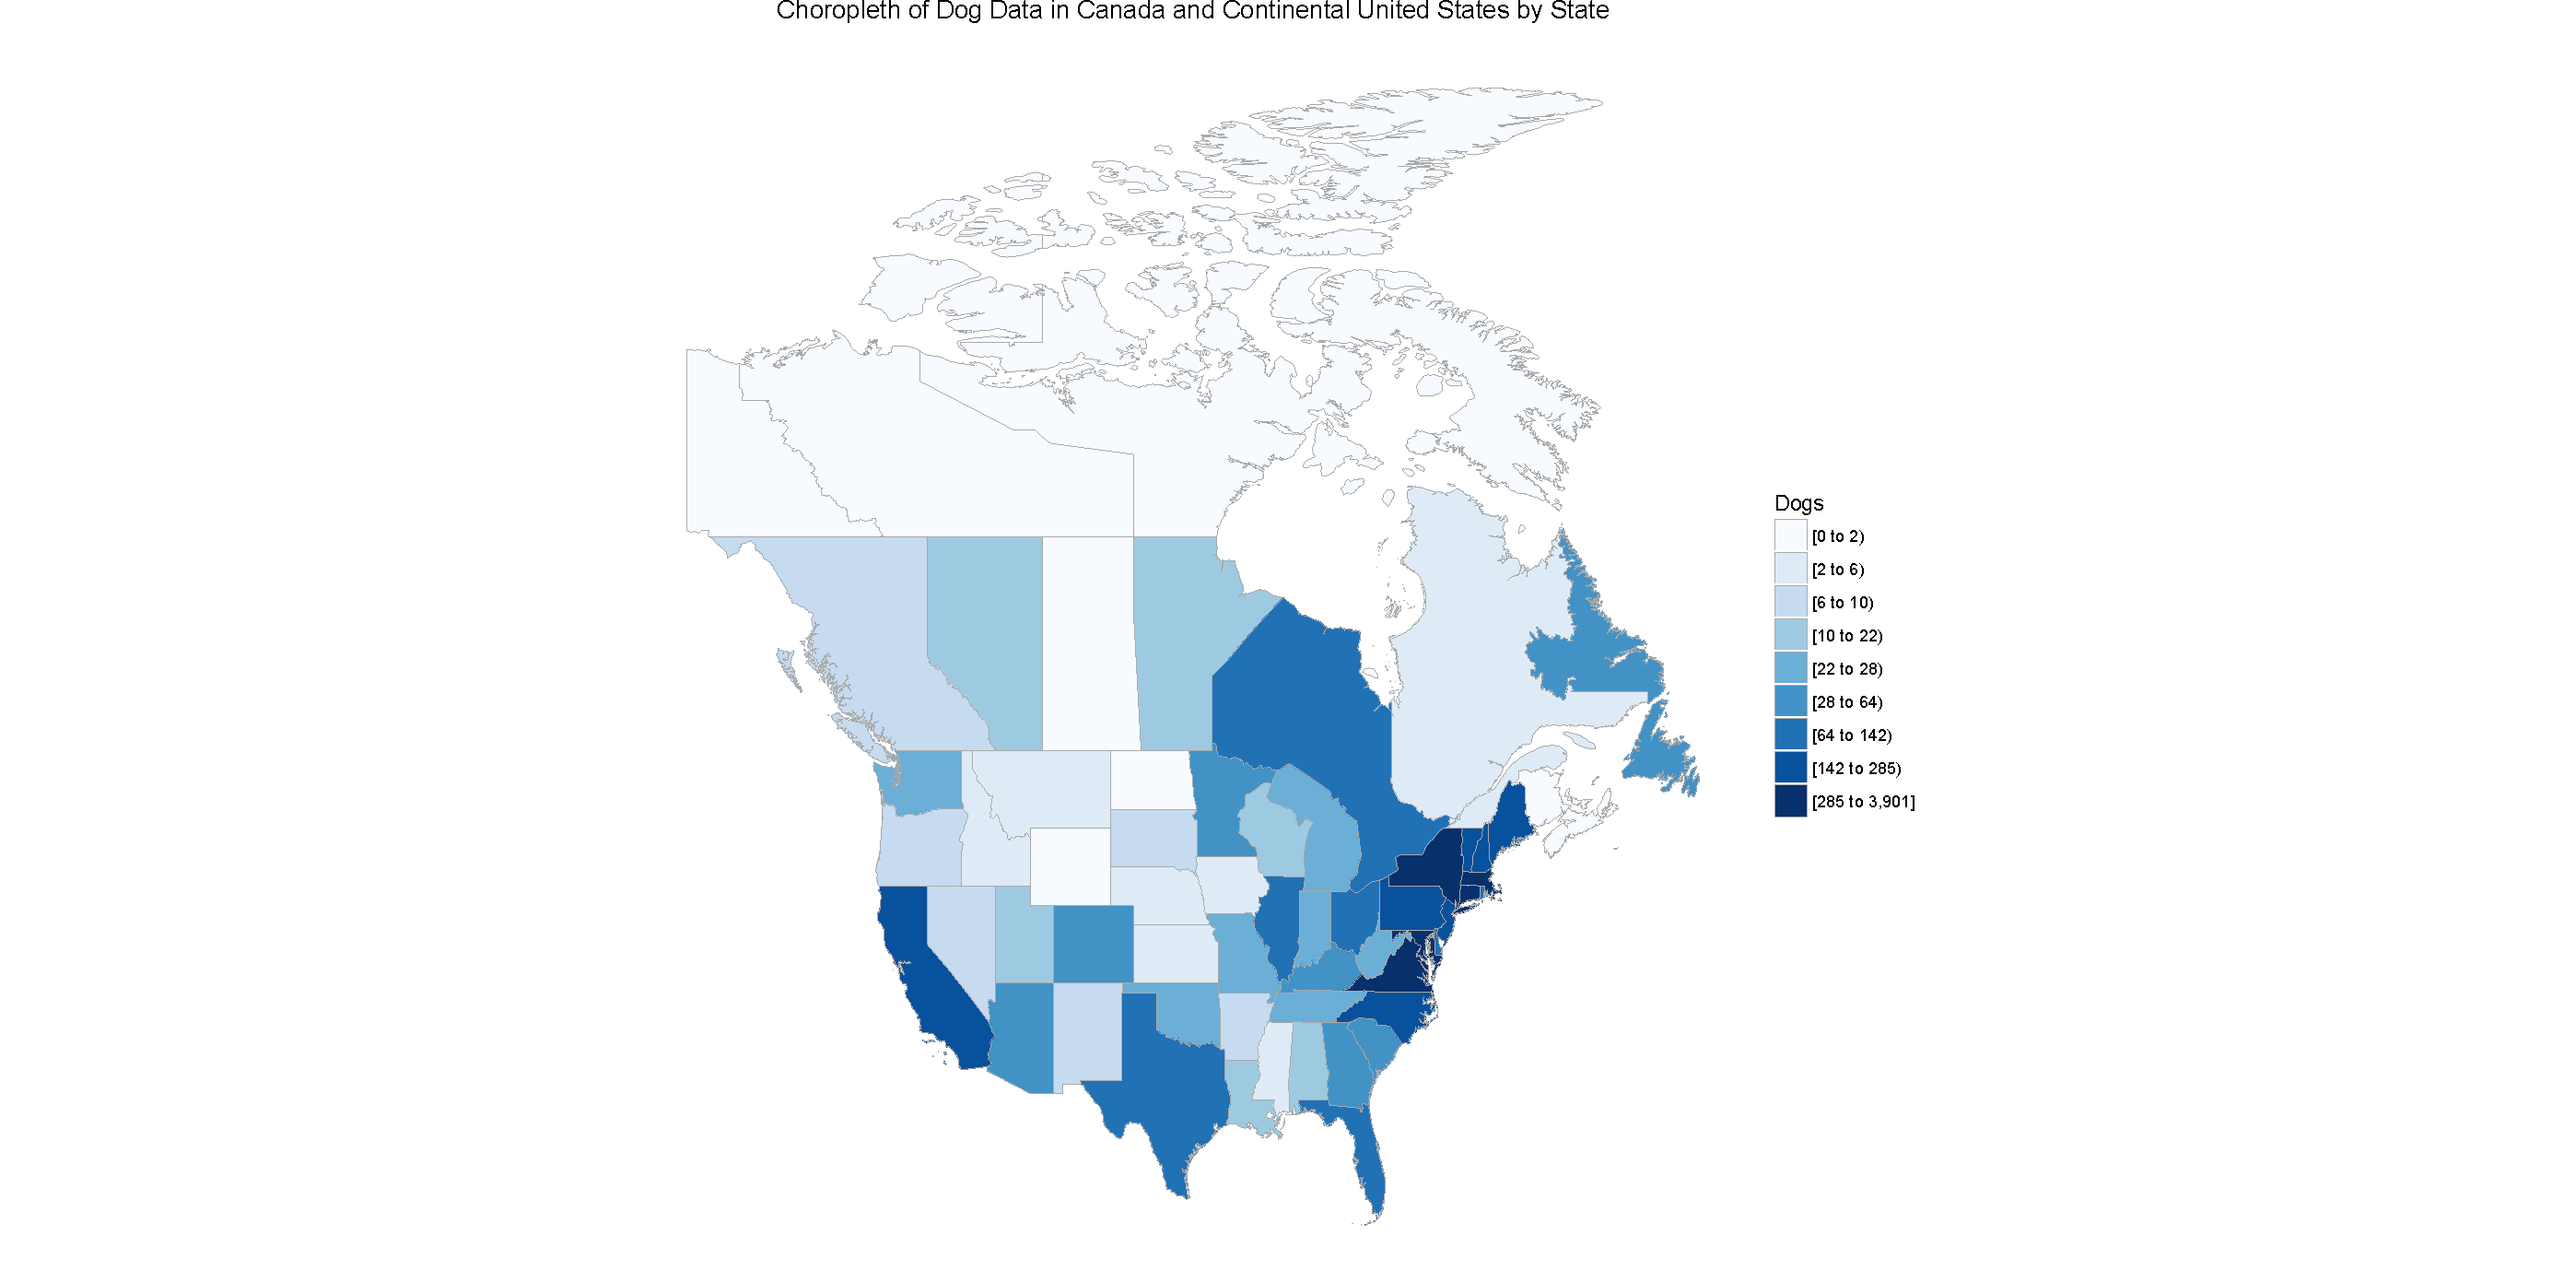
\includegraphics[width=1.3\textwidth]{Choro_Dog.pdf}
\centering

\end{figure}

\end{frame}

\begin{frame}{Choropleth of Dog Data in Northeast}
\begin{figure}
\centering
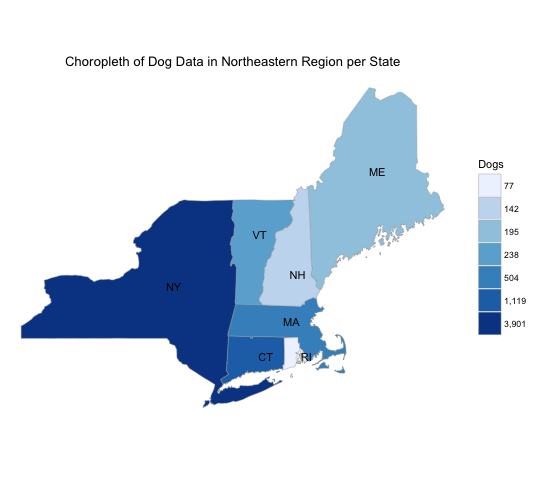
\includegraphics[width=.9\textwidth]{Choropleth_NE_US.png}
\end{figure}

\end{frame}

\begin{frame}{Choropleth by Zip Code NY}
\centering
\begin{figure}
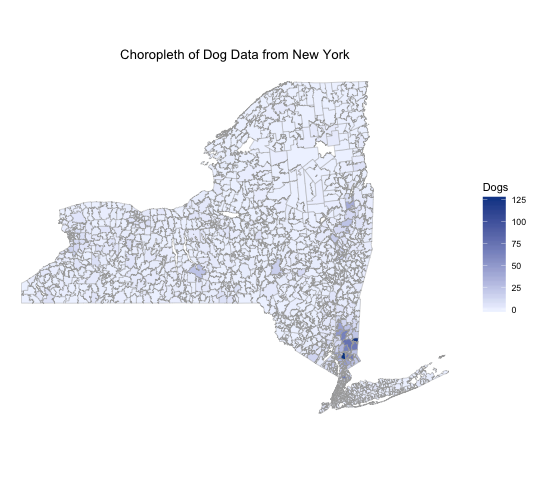
\includegraphics[width=.9\textwidth]{New_York_Choropleth.png}
\end{figure}

\end{frame}

\subsection{Choropleth Map in R Using Zip Codes}
\begin{frame}{Choropleths in R}
To create this map, we:
\begin{itemize}

\item Installed packages that allow R to work with zip codes, states, and regions, and use GGPlot to create choropleth maps, which are used to display themes such as population density
\item Created maps of US states with Canadian provinces, zoomed in on Northeastern US states, and created another map using New York zip codes
\item Packages used: choroplethr, choroplethrMaps, choroplethrZip, admin1\_region\_choropleth 
\end{itemize}

\end{frame}

\subsection{ggplot}

\begin{frame}{Truncated Data}
\begin{figure}
\centering
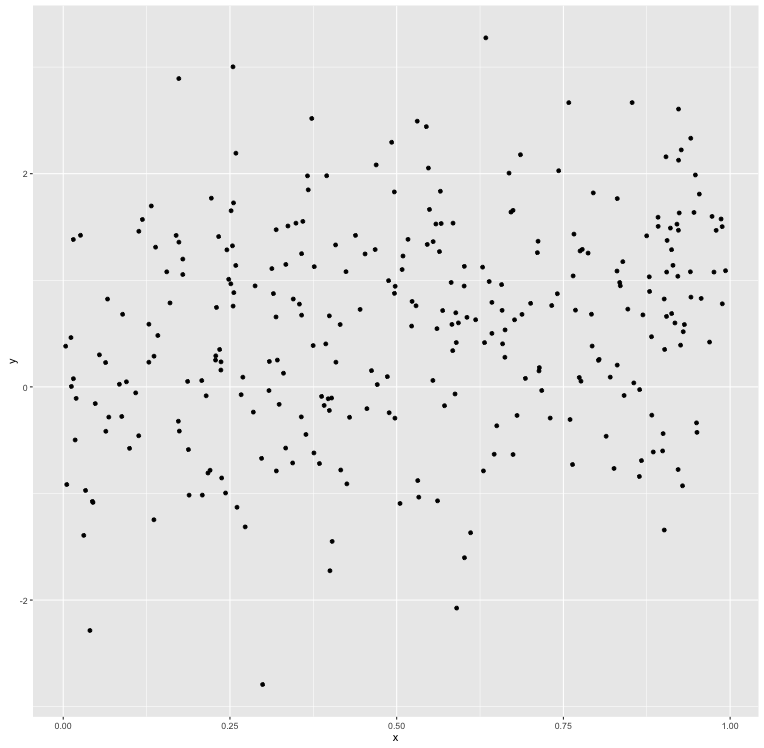
\includegraphics[width=.7\textwidth]{plot_zoom_png-2.png}
\end{figure}



\end{frame}

\begin{frame}{Truncated Data}
\begin{figure}
\centering
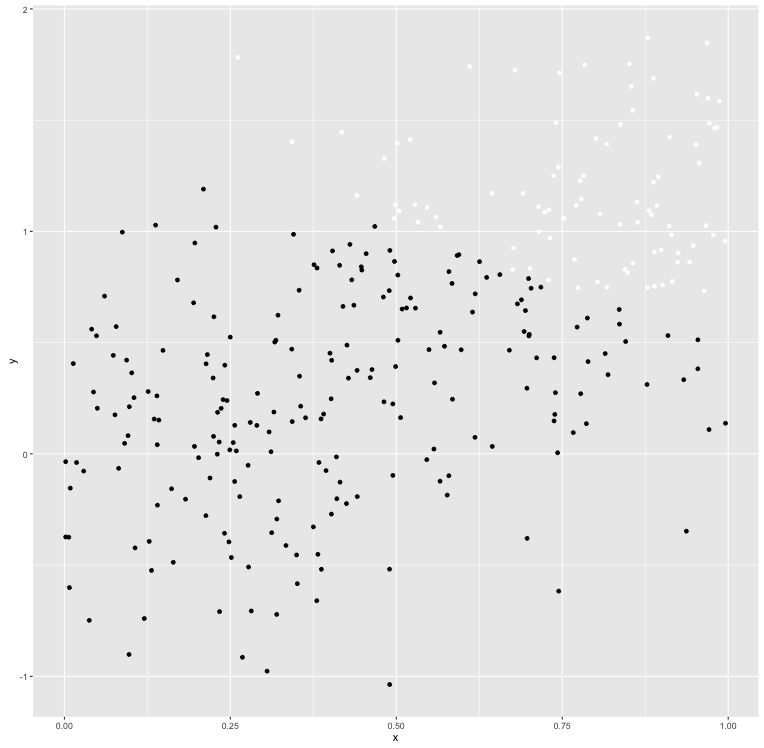
\includegraphics[width=.7\textwidth]{plot_zoom_png-3.png}

\end{figure}

\end{frame}

\begin{frame}{Diagnosis Age by Date of Birth}

\begin{figure}
\centering
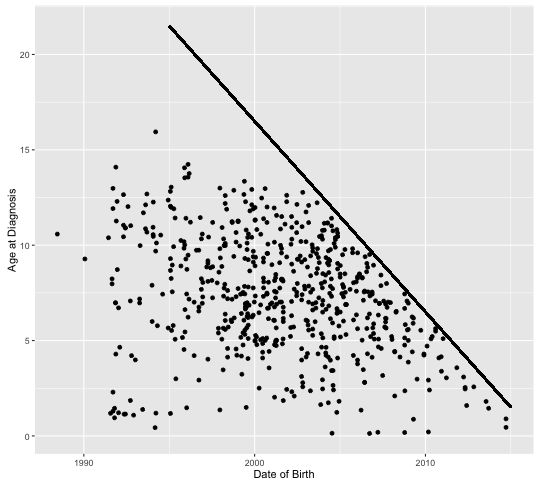
\includegraphics[width=.7\textwidth]{Dog_Data_Scatterplot.png}

\end{figure}

\end{frame}

\begin{frame}{Truncated Random Variables}

A truncated distribution means that at a certain point, the data is cut short, and we do not have complete information about one end of the distribution, as it cannot be observed
\vskip.5cm

In our case, our data is truncated. As we approach the current year, any dogs born in recent years who are diagnosed with cancer are only diagnosed at younger years. For example, given a dog born in 2014 and diagnosed with cancer in its lifetime, it will only be in our data if its diagnosed by the age of two years old. If it will be diagnosed at a later age, we do not have that information yet.
\vskip.5cm

\end{frame}

\begin{frame}{Truncated Random Variables}

Our scatterplot of the data makes it seem as though the age of diagnosis has gotten younger over the past decade. This is a false trend because, in reality, dogs that have been born recently cannot be diagnosed with cancer at older ages yet. Although they may develop MCT later in life, we do not have this data, so we cannot make conclusions taking our current data at face value.

\end{frame}



\section{Future Work}

\begin{frame}{Future Work}

In general, we want to test the hypothesis that dogs are being diagnosed with cancer at younger ages as years pass. To do this, we have to use statistical tools to account for this truncated data while focus on modeling the data we have from earlier years of the study. We can then focus on analyzing this claim using statistical models to allow us to predict the age of diagnosis for dogs that will develop MCT in the future.

\end{frame}

\end{document}